\section{Experimentos}
Apresento aqui os experimentos e testes realizados para os grafos inseridos.
\subsection{Experimento 01}

Dado o seguinte grafo, devemos encontrar apenas um único caminho disjunto, sendo ele [A $\rightarrow$ C $\rightarrow$ D] pelo fato do caminho disjunto, quando único, ser o menor caminho possível.

\begin{center}
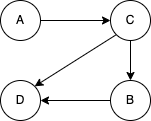
\includegraphics[width=5cm, height=4cm]{figuras/01.png}
\end{center}

O Algoritmo implementado teve o seguinte resultado:

\begin{scriptsize}
\estiloR
\begin{lstlisting}[title={Exemplo 01}, label=lst:javacode]
 == Exemplo 01 == 
0 -> 2 -> 3
Caminhos disjuntos encontrados: 1 
\end{lstlisting}
\end{scriptsize}

\subsection{Experimento 02}

Dado o seguinte grafo, devemos encontrar dois caminhos disjuntos, sendo eles [1 $\rightarrow$ 2 $\rightarrow$ 4] e [1 $\rightarrow$ 3 $\rightarrow$ 4]

\begin{center}
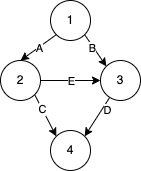
\includegraphics[height=4cm]{figuras/02.png}
\end{center}

O Algoritmo implementado teve o seguinte resultado:

\begin{scriptsize}
\estiloR
\begin{lstlisting}[title={Exemplo 02}, label=lst:javacode]
 == Exemplo 02 == 
0 -> 1 -> 3
0 -> 2 -> 3
Caminhos disjuntos encontrados: 2 
\end{lstlisting}
\end{scriptsize}

\subsection{Experimento 03}

Dado o seguinte grafo, devemos encontrar três caminhos disjuntos, sendo eles [1 -> 2 -> 8] e [1 -> 5 -> 8] e [1 -> 3 -> 7 -> 8]

\begin{center}
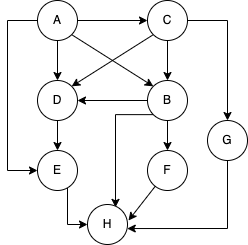
\includegraphics[height=4cm]{figuras/03.png}
\end{center}

e o grafo desenhado com os caminhos que devem ser encontrados:

\begin{center}
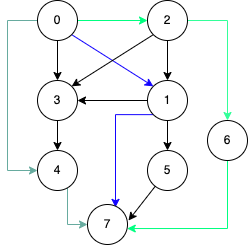
\includegraphics[height=6cm]{figuras/03_caminhos.png}
\end{center}


O Algoritmo implementado teve o seguinte resultado:

\begin{scriptsize}
\estiloR
\begin{lstlisting}[title={Exemplo 03}, label=lst:javacode]
 == Exemplo 03 == 
0 -> 1 -> 7
0 -> 4 -> 7
0 -> 2 -> 6 -> 7
Caminhos disjuntos encontrados: 3 
\end{lstlisting}
\end{scriptsize}


\subsection{Experimento 04}

Dado o seguinte grafo, devemos encontrar dois caminhos disjuntos, sendo eles 
[0 -> 1 ]

\begin{center}
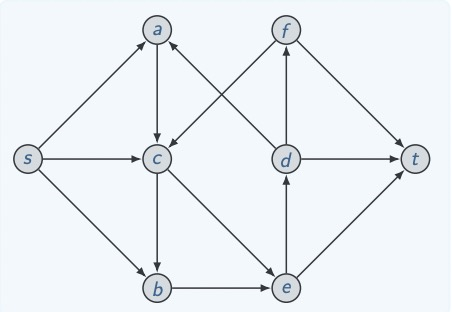
\includegraphics[height=4cm]{figuras/04.jpg}
\end{center}

e o grafo desenhado com os caminhos que devem ser encontrados (conforme no slide da aula):

\begin{center}
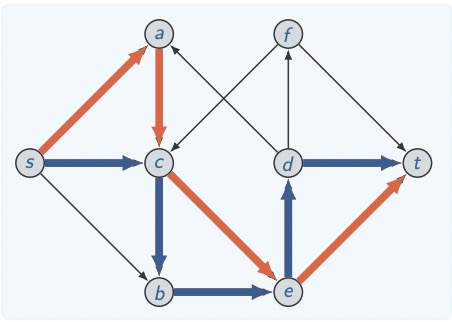
\includegraphics[height=6cm]{figuras/04_caminhos.jpg}
\end{center}

entretanto, o algoritmo encontrou outros possíveis caminhos:

\begin{center}
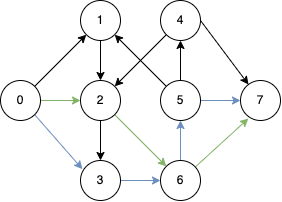
\includegraphics[height=6cm]{figuras/04_caminhos2.png}
\end{center}



O Algoritmo implementado teve o seguinte resultado:

\begin{scriptsize}
\estiloR
\begin{lstlisting}[title={Exemplo 04}, label=lst:javacode]
 == Exemplo 04 == 
0 -> 2 -> 6 -> 7
0 -> 3 -> 6 -> 5 -> 7
Caminhos disjuntos encontrados: 2 
\end{lstlisting}
\end{scriptsize}


\section{Resultados Obtidos}

Implementei um algoritmo usando a base do Fork-Fulkerson com grafo residual e pesos 0 nas arestas para que não haja repetição das mesmas e uma busca em largura como um algoritmo de busca para encontrar os caminhos, seguindo pela lógica arestas ja visitadas e pesoso para um possível futura implementação nesse código.

O algoritmo está funcionando, vários testes foram feitos, inclusive utilizando um problema apresentado em aula chegando também em dois caminhos disjuntos diferentes, mas possíveis dentro do problema em questão.
